% Options for packages loaded elsewhere
\PassOptionsToPackage{unicode}{hyperref}
\PassOptionsToPackage{hyphens}{url}
\PassOptionsToPackage{dvipsnames,svgnames,x11names}{xcolor}
%
\documentclass[
  letterpaper,
  DIV=11,
  numbers=noendperiod]{scrartcl}

\usepackage{amsmath,amssymb}
\usepackage{iftex}
\ifPDFTeX
  \usepackage[T1]{fontenc}
  \usepackage[utf8]{inputenc}
  \usepackage{textcomp} % provide euro and other symbols
\else % if luatex or xetex
  \usepackage{unicode-math}
  \defaultfontfeatures{Scale=MatchLowercase}
  \defaultfontfeatures[\rmfamily]{Ligatures=TeX,Scale=1}
\fi
\usepackage{lmodern}
\ifPDFTeX\else  
    % xetex/luatex font selection
\fi
% Use upquote if available, for straight quotes in verbatim environments
\IfFileExists{upquote.sty}{\usepackage{upquote}}{}
\IfFileExists{microtype.sty}{% use microtype if available
  \usepackage[]{microtype}
  \UseMicrotypeSet[protrusion]{basicmath} % disable protrusion for tt fonts
}{}
\makeatletter
\@ifundefined{KOMAClassName}{% if non-KOMA class
  \IfFileExists{parskip.sty}{%
    \usepackage{parskip}
  }{% else
    \setlength{\parindent}{0pt}
    \setlength{\parskip}{6pt plus 2pt minus 1pt}}
}{% if KOMA class
  \KOMAoptions{parskip=half}}
\makeatother
\usepackage{xcolor}
\setlength{\emergencystretch}{3em} % prevent overfull lines
\setcounter{secnumdepth}{5}
% Make \paragraph and \subparagraph free-standing
\makeatletter
\ifx\paragraph\undefined\else
  \let\oldparagraph\paragraph
  \renewcommand{\paragraph}{
    \@ifstar
      \xxxParagraphStar
      \xxxParagraphNoStar
  }
  \newcommand{\xxxParagraphStar}[1]{\oldparagraph*{#1}\mbox{}}
  \newcommand{\xxxParagraphNoStar}[1]{\oldparagraph{#1}\mbox{}}
\fi
\ifx\subparagraph\undefined\else
  \let\oldsubparagraph\subparagraph
  \renewcommand{\subparagraph}{
    \@ifstar
      \xxxSubParagraphStar
      \xxxSubParagraphNoStar
  }
  \newcommand{\xxxSubParagraphStar}[1]{\oldsubparagraph*{#1}\mbox{}}
  \newcommand{\xxxSubParagraphNoStar}[1]{\oldsubparagraph{#1}\mbox{}}
\fi
\makeatother


\providecommand{\tightlist}{%
  \setlength{\itemsep}{0pt}\setlength{\parskip}{0pt}}\usepackage{longtable,booktabs,array}
\usepackage{calc} % for calculating minipage widths
% Correct order of tables after \paragraph or \subparagraph
\usepackage{etoolbox}
\makeatletter
\patchcmd\longtable{\par}{\if@noskipsec\mbox{}\fi\par}{}{}
\makeatother
% Allow footnotes in longtable head/foot
\IfFileExists{footnotehyper.sty}{\usepackage{footnotehyper}}{\usepackage{footnote}}
\makesavenoteenv{longtable}
\usepackage{graphicx}
\makeatletter
\def\maxwidth{\ifdim\Gin@nat@width>\linewidth\linewidth\else\Gin@nat@width\fi}
\def\maxheight{\ifdim\Gin@nat@height>\textheight\textheight\else\Gin@nat@height\fi}
\makeatother
% Scale images if necessary, so that they will not overflow the page
% margins by default, and it is still possible to overwrite the defaults
% using explicit options in \includegraphics[width, height, ...]{}
\setkeys{Gin}{width=\maxwidth,height=\maxheight,keepaspectratio}
% Set default figure placement to htbp
\makeatletter
\def\fps@figure{htbp}
\makeatother
% definitions for citeproc citations
\NewDocumentCommand\citeproctext{}{}
\NewDocumentCommand\citeproc{mm}{%
  \begingroup\def\citeproctext{#2}\cite{#1}\endgroup}
\makeatletter
 % allow citations to break across lines
 \let\@cite@ofmt\@firstofone
 % avoid brackets around text for \cite:
 \def\@biblabel#1{}
 \def\@cite#1#2{{#1\if@tempswa , #2\fi}}
\makeatother
\newlength{\cslhangindent}
\setlength{\cslhangindent}{1.5em}
\newlength{\csllabelwidth}
\setlength{\csllabelwidth}{3em}
\newenvironment{CSLReferences}[2] % #1 hanging-indent, #2 entry-spacing
 {\begin{list}{}{%
  \setlength{\itemindent}{0pt}
  \setlength{\leftmargin}{0pt}
  \setlength{\parsep}{0pt}
  % turn on hanging indent if param 1 is 1
  \ifodd #1
   \setlength{\leftmargin}{\cslhangindent}
   \setlength{\itemindent}{-1\cslhangindent}
  \fi
  % set entry spacing
  \setlength{\itemsep}{#2\baselineskip}}}
 {\end{list}}
\usepackage{calc}
\newcommand{\CSLBlock}[1]{\hfill\break\parbox[t]{\linewidth}{\strut\ignorespaces#1\strut}}
\newcommand{\CSLLeftMargin}[1]{\parbox[t]{\csllabelwidth}{\strut#1\strut}}
\newcommand{\CSLRightInline}[1]{\parbox[t]{\linewidth - \csllabelwidth}{\strut#1\strut}}
\newcommand{\CSLIndent}[1]{\hspace{\cslhangindent}#1}

\usepackage{float}
\usepackage{tabularray}
\usepackage[normalem]{ulem}
\usepackage{graphicx}
\UseTblrLibrary{booktabs}
\UseTblrLibrary{rotating}
\UseTblrLibrary{siunitx}
\NewTableCommand{\tinytableDefineColor}[3]{\definecolor{#1}{#2}{#3}}
\newcommand{\tinytableTabularrayUnderline}[1]{\underline{#1}}
\newcommand{\tinytableTabularrayStrikeout}[1]{\sout{#1}}
\KOMAoption{captions}{tableheading}
\makeatletter
\@ifpackageloaded{caption}{}{\usepackage{caption}}
\AtBeginDocument{%
\ifdefined\contentsname
  \renewcommand*\contentsname{Table of contents}
\else
  \newcommand\contentsname{Table of contents}
\fi
\ifdefined\listfigurename
  \renewcommand*\listfigurename{List of Figures}
\else
  \newcommand\listfigurename{List of Figures}
\fi
\ifdefined\listtablename
  \renewcommand*\listtablename{List of Tables}
\else
  \newcommand\listtablename{List of Tables}
\fi
\ifdefined\figurename
  \renewcommand*\figurename{Figure}
\else
  \newcommand\figurename{Figure}
\fi
\ifdefined\tablename
  \renewcommand*\tablename{Table}
\else
  \newcommand\tablename{Table}
\fi
}
\@ifpackageloaded{float}{}{\usepackage{float}}
\floatstyle{ruled}
\@ifundefined{c@chapter}{\newfloat{codelisting}{h}{lop}}{\newfloat{codelisting}{h}{lop}[chapter]}
\floatname{codelisting}{Listing}
\newcommand*\listoflistings{\listof{codelisting}{List of Listings}}
\makeatother
\makeatletter
\makeatother
\makeatletter
\@ifpackageloaded{caption}{}{\usepackage{caption}}
\@ifpackageloaded{subcaption}{}{\usepackage{subcaption}}
\makeatother

\ifLuaTeX
  \usepackage{selnolig}  % disable illegal ligatures
\fi
\usepackage{bookmark}

\IfFileExists{xurl.sty}{\usepackage{xurl}}{} % add URL line breaks if available
\urlstyle{same} % disable monospaced font for URLs
\hypersetup{
  pdftitle={Focasting The Trend of Vehicle Related Crime In Calgary In 2025},
  pdfauthor={Haobo Ren},
  colorlinks=true,
  linkcolor={blue},
  filecolor={Maroon},
  citecolor={Blue},
  urlcolor={Blue},
  pdfcreator={LaTeX via pandoc}}


\title{Focasting The Trend of Vehicle Related Crime In Calgary In
2025\thanks{Code and data are available at:
https://github.com/HaoboRrrr/calgary\_vehicle\_crime\_forcast}}
\usepackage{etoolbox}
\makeatletter
\providecommand{\subtitle}[1]{% add subtitle to \maketitle
  \apptocmd{\@title}{\par {\large #1 \par}}{}{}
}
\makeatother
\subtitle{An Analysis of Calgary's Crime Count From 2018 to 2024}
\author{Haobo Ren}
\date{November 23, 2024}

\begin{document}
\maketitle
\begin{abstract}
Vehicle-related crime is a long-standing challenge to urban security, so
accurate prediction is necessary to effectively allocate police
resources and develop security policies. This study examines trends in
vehicle-related crime in Calgary, Canada, focusing on two types of
crime: Theft of vehicle and Theft from vehicle. A Bayesian regression
model is fit to historical crime data from January 2018 to October 2024,
accounting for seasonal variations (months), long-term trends (years),
and differences between crime categories. The usefulness of Bayesian
modeling for crime trend forecasting is demonstrated by this analysis,
providing law enforcement and policymakers practical insights to foresee
and handle long-term and seasonal crime trends.
\end{abstract}


\section{Introduction}\label{introduction}

Urban crime is an ongoing problem compromising public confidence,
economic stability, and safety. Among the several types of crimes,
vehicle-related offenses include theft of vehicles and theft from
vehicles remain a major issue in urban areas across the country. These
crimes disturb people's life but also burden local governments and law
enforcement. Over the years, Calgary, Canada, has seen varying patterns
in vehicle-related crimes, which raises issues regarding future
developments of these trends. Designing effective preventive plans,
maximizing resource allocation, and guaranteeing community safety all
depend on an awareness of current trends and future crime count
prediction. This study forecasts vehicle-related crime patterns in
Calgary up until 2025, therefore addressing these issues.

Analyzing and projecting monthly crime counts for theft from vehicles
and theft of vehicles in Calgary is the main aim of this study. I
created a Bayesian regression model to assess the effects of time (year
and month) and crime category on reported crime counts using historical
data spanning January 2018 through October 2024. Offering a
comprehensive knowledge of how vehicle-related crimes have developed and
may continue to alter in the near future, the model catches both
long-term patterns and seasonal changes. The research also offers
category-specific forecasts, therefore stressing variations in the
seasonal and temporal trends of theft from and of vehicles.

The analysis reveals a continued decline in vehicle-related crimes in
Calgary, with a mean change of -60.4 each year, and notable mean
differences of -435.0 between the two categories. Theft from vehicles is
anticipated to show cyclical surges in the summer months, indicating
possible opportunistic habits. Conversely, vehicle theft exhibits a more
stable decline throughout the course of the year. The data indicate
that, although overall vehicle-related crimes are down, seasonal surges
in certain categories persist as a problem for policymakers and law
enforcement to tackle, for example, the crime count of Theft From
Vehicle in August is expected larger than January by 158.4.

The study is significant for its role in proactive crime prevention and
resource optimization. This study offers precise and comprehensible
forecasts, providing policymakers and law enforcement with
evidence-based insights to inform decision-making. This study addresses
a significant research gap and enhances public safety in Calgary.

\#Telegraphing paragraph: The remainder of this paper is structured as
follows. Section~\ref{sec-data}\ldots.

\section{Data}\label{sec-data}

\subsection{Overview}\label{overview}

The raw dataset obtained from Open Data Calgary(Calgary, n.d.) was
recorded and updated monthly by the Calgary Police Service. The data is
considered cumulative as late-reported incidents are often received well
after an offence has occurred. An incident is either reported just after
the crime happened, or reported on the Calgary Police Service(Service,
n.d.).

The data analysis and visualization is done in R(R Core Team 2023) with
the following Packages: tidyverse(Wickham et al. 2019), janitor(Firke
2023), arrow(Richardson et al. 2024), rstanarm(Goodrich et al. 2022),
ggplot2(Wickham 2016), dplyr(Wickham et al. 2022), here, knitr.

\subsection{Measurement}\label{measurement}

The data reflects reported crime incidents across Calgary, categorized
by community, crime type, and temporal details (year and month). Each
row in the dataset represents a summary of crime counts for a specific
category and community within a given month and year. The Calgary Police
Service serves as the primary source, systematically recording incidents
reported by the public. These reports may be filed in several ways,
including: immediate Reporting and delayed Reporting.

Crime count quantifies the number of reported incidents of a specific
crime and time period and is based on the most serious violation per
incident. The count represents and aggregation of individual reports
collected by the Calgary Police Services.

There are limitations in these measurement. Reporting Bias: Not all
crimes are reported. Minor incidents or those involving uninsured
vehicles may go unreported, leading to underestimation of true crime
rates. Cumulative Nature: The inclusion of late-reported incidents makes
it challenging to distinguish between crimes that occurred during the
reported month versus those that occurred earlier.

By understanding how this dataset measures real-world crime phenomena,
we can more confidently interpret the insights and predictions derived
from it.

\subsection{Data Examination}\label{sec-dataexam}

The raw data from Open Data has five columns and 75,595 rows, the column
names are displayed below:

\begin{longtable}[]{@{}l@{}}
\toprule\noalign{}
column\_names \\
\midrule\noalign{}
\endhead
\bottomrule\noalign{}
\endlastfoot
Community \\
Category \\
Crime Count \\
Year \\
Month \\
\end{longtable}

\begin{itemize}
\tightlist
\item
  Community: The dataset is spatially disaggregated into Calgary's
  various communities
\end{itemize}

Numeric Variable:

\begin{itemize}
\tightlist
\item
  Year: The year of each record indicate when the incidents were
  reported.
\end{itemize}

Categorical Variable:

\begin{itemize}
\item
  Category: Each entry is categorized into distinct crime types.
\item
  month: The month of each incidents recorded. Range from 1-12
  repeatedly each year
\end{itemize}

Response Variable:

\begin{itemize}
\tightlist
\item
  Crime Count: This variable quantifies the number of reported incidents
  of a specific crime type (e.g., theft from or of vehicles) within a
  given community and time period.
\end{itemize}

\subsection{Data Cleaning}\label{data-cleaning}

Several steps was taken for better analysis of vehicle-related trend in
Calgary. First, clean the names of all the columns. Second, the raw
dataset contained granular records categorized by Community and specific
details. These were aggregated to provide summarized counts of crimes
(crime\_count) by category, year, and month to align with analysis
requirements. Third, a new time column was introduced in the cleaned
data, combining year and month into a single date field (YYYY-MM-DD).
This was essential for time-series analysis and visualization. Last,
filter out the categories related to vehicle.

\subsection{Cleaned Data}\label{cleaned-data}

The first 6 rows of the cleaned dataset are shown in
Table~\ref{tbl-cleaned-data}.

\begin{longtable}[]{@{}lrrrl@{}}

\caption{\label{tbl-cleaned-data}Head of cleaned Calgary Crime data}

\tabularnewline

\toprule\noalign{}
category & crime\_count & year & month & time \\
\midrule\noalign{}
\endhead
\bottomrule\noalign{}
\endlastfoot
Theft FROM Vehicle & 962 & 2018 & 1 & 2018-01-01 \\
Theft FROM Vehicle & 645 & 2018 & 2 & 2018-02-01 \\
Theft FROM Vehicle & 818 & 2018 & 3 & 2018-03-01 \\
Theft FROM Vehicle & 870 & 2018 & 4 & 2018-04-01 \\
Theft FROM Vehicle & 1063 & 2018 & 5 & 2018-05-01 \\
Theft FROM Vehicle & 1036 & 2018 & 6 & 2018-06-01 \\

\end{longtable}

\subsection{Response Variable}\label{response-variable}

\subsubsection{Crime count of Theft FROM
Vehicle}\label{crime-count-of-theft-from-vehicle}

Summary statistics of Crime count of Theft FROM Vehicle are shown in the
Table~\ref{tbl-response-theftfromvehicle}

\begin{longtable}[]{@{}ll@{}}

\caption{\label{tbl-response-theftfromvehicle}Summary Statitic of
crime\_count(Theft FROM Vehicle)}

\tabularnewline

\toprule\noalign{}
& crime\_count \\
\midrule\noalign{}
\endhead
\bottomrule\noalign{}
\endlastfoot
& Min. : 120.0 \\
& 1st Qu.: 788.2 \\
& Median : 916.0 \\
& Mean : 932.7 \\
& 3rd Qu.:1105.5 \\
& Max. :1619.0 \\

\end{longtable}

The response variable, crime\_count, represents the number of reported
incidents of theft from vehicles within Calgary. The summary statistics
reveal a significant variability in the crime counts, ranging from a
minimum of 120 to a maximum of 1,619 reported cases. The median value is
916, indicating that half of the recorded months experienced fewer than
916 thefts, while the other half exceeded this value. The mean crime
count, at 932.7, is slightly higher than the median, suggesting the
presence of months with particularly high crime counts that may be
skewing the average. The interquartile range (IQR), spanning from 788.2
(1st quartile) to 1,105.5 (3rd quartile), highlights the central
tendency of crime occurrences, with most months falling within this
range. These statistics emphasize the fluctuating nature of vehicle
thefts in Calgary and provide a foundational understanding for modeling
and forecasting future trends.

\subsubsection{Crime count of Theft OF
Vehicle}\label{crime-count-of-theft-of-vehicle}

Summary statistics of Crime count of Theft FROM Vehicle are shown in the
Table~\ref{tbl-response-theftofvehicle}

\begin{longtable}[]{@{}ll@{}}

\caption{\label{tbl-response-theftofvehicle}Summary Statitic of
crime\_count(Theft OF Vehicle)}

\tabularnewline

\toprule\noalign{}
& crime\_count \\
\midrule\noalign{}
\endhead
\bottomrule\noalign{}
\endlastfoot
& Min. :146.0 \\
& 1st Qu.:361.2 \\
& Median :424.5 \\
& Mean :422.5 \\
& 3rd Qu.:469.0 \\
& Max. :651.0 \\

\end{longtable}

The response variable, crime\_count, for Theft OF Vehicle incidents
reflects the monthly reported counts of vehicles being stolen in
Calgary. The dataset's summary statistics indicate that the crime counts
range from a minimum of 146 to a maximum of 651 incidents. The median
count is 424.5, suggesting that half of the months have fewer than 425
thefts, while the other half exceed this value. Interestingly, the mean
crime count is 422.5, closely aligned with the median, suggesting a
relatively symmetric distribution of the data. The interquartile range
(IQR) spans from 361.2 (1st quartile) to 469.0 (3rd quartile),
indicating that most monthly counts are concentrated within this range.
These figures highlight the scale and regularity of vehicle theft in
Calgary and form an essential basis for analyzing and forecasting trends
in such crimes.

\subsection{Predictor Variable}\label{predictor-variable}

\subsubsection{year}\label{year}

The variable year represents the timeline over which the crime data is
recorded, providing insight into how vehicle-related crime counts have
changed annually. By analyzing the data across different years, we can
observe any long-term trends, such as consistent increases, decreases,
or fluctuations in vehicle thefts. This variable helps us understand
whether certain years experienced higher crime rates due to factors like
economic conditions, population changes, or other external influences.

\subsubsection{month and category}\label{month-and-category}

The variables month and category provide a detailed view of how
vehicle-related crimes are distributed across time and crime types.
Month captures seasonal variations, showing how crime rates fluctuate
throughout the year. For example, there might be a tendency for higher
crime counts during certain seasons, such as summer or winter,
influenced by weather conditions or holiday activities. Category
distinguishes between ``Theft FROM Vehicle'' and ``Theft OF Vehicle,''
allowing us to compare the frequency and patterns of these two crime
types. Together, these variables highlight differences in the nature and
timing of vehicle-related crimes, offering valuable insights into their
temporal and categorical distributions.

\subsection{Trend of The Two Crime}\label{trend-of-the-two-crime}

The trend of Theft FROM Vehicle and Theft OF Vehicle are shown in
Figure~\ref{fig-combined-trend}

\begin{figure}

\centering{

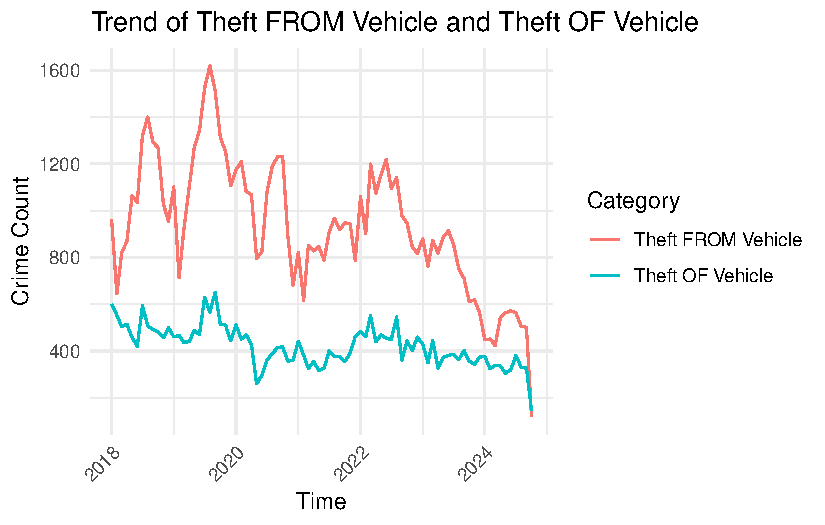
\includegraphics{paper_files/figure-pdf/fig-combined-trend-1.pdf}

}

\caption{\label{fig-combined-trend}Trend of The Two Crime Combined}

\end{figure}%

\newpage

The trends for ``Theft FROM Vehicle'' and ``Theft OF Vehicle'' reveal
distinct patterns over time. ``Theft FROM Vehicle'' consistently shows
higher crime counts compared to ``Theft OF Vehicle,'' indicating that it
is a more prevalent issue. The trend for ``Theft FROM Vehicle''
demonstrates significant fluctuations, with peaks around 2019 and a
general decline afterward, suggesting a reduction in these incidents in
more recent years. In contrast, ``Theft OF Vehicle'' exhibits a
relatively stable pattern with smaller variations over time. Although it
remains less frequent than ``Theft FROM Vehicle,'' its counts appear to
decrease gradually, particularly after 2022. Both categories show
declining trends toward the end of the observed period, which could
reflect successful crime prevention measures or other external
influences.

\section{Model}\label{model}

The Bayesian regression model was developed to analyze and forecast the
trends of vehicle-related crimes in Calgary, focusing on the categories
``Theft FROM Vehicle'' and ``Theft OF Vehicle.'' The primary goal of
this modeling is to understand the relationship between crime counts and
key predictors such as time (year and month) and crime categories, as
well as their interactions. By incorporating temporal and categorical
variables, the model seeks to capture long-term trends, seasonal
patterns, and differences between the two types of crimes. Ultimately,
the model provides a foundation for projecting future crime rates,
offering valuable insights that can support strategic decision-making
and the development of targeted crime prevention initiatives for 2025
and beyond.

Background details and diagnostics are included in
\textbf{?@sec-model-details}.

\subsection{Model set-up}\label{model-set-up}

The Bayesian regression model is set up to examine the relationship
between vehicle-related crime counts and the selected predictors. The
response variable, \(y_i\), represents the observed crime count for the
i-th observation, where each observation corresponds to a specific
month, year, and crime category. The predictors include a numeric
variable for year, categorical variables for month and category, as well
as interaction terms (category:month and category:year) to capture how
crime patterns differ between the two crime types over time and across
seasons.

The model assumes the form:

\[
y_i = \beta_0 + \beta_1 \text{year}_i + \beta_2 \text{month}_i + \beta_3 \text{category}_i + \beta_4 (\text{category} \times \text{month})_i + \beta_5 (\text{category} \times \text{year})_i + \epsilon_i
\]

Here, \(\beta_0\) is the intercept, capturing the baseline level of
crime counts. The coefficients \(\beta_1\), \(\beta_2\), and \(\beta_3\)
quantify the effects of year, month, and category, respectively, while
\(\beta_4\) and \(\beta_5\) capture the interaction effects. The error
term \(\epsilon_i\) accounts for the residual variability in crime
counts not explained by the predictors, modeled with a Gaussian
distribution. This setup allows the model to estimate the relative
contributions of each predictor to crime counts and their combined
effects on the observed trends.

\subsection{Model justification}\label{model-justification}

The primary goal of this model is to forecast trends in vehicle-related
crimes in Calgary, focusing on two categories: ``Theft FROM Vehicle''
and ``Theft OF Vehicle.'' To achieve this, a Bayesian regression model
was chosen, as it provides a robust framework for incorporating prior
knowledge, handling uncertainty, and capturing complex relationships
between predictors.

The selection of predictors for the Bayesian regression model is
grounded in their expected relationship with the response variable,
crime\_count, and their importance in explaining and forecasting trends
in vehicle-related crimes. Below is a detailed justification for each
predictor.

\subsubsection{year(Numeric Predictor)}\label{yearnumeric-predictor}

The year variable is included as a numeric predictor because
vehicle-related crimes are likely influenced by long-term trends over
time. For instance, crime rates may decrease due to improvements in law
enforcement strategies or community awareness campaigns. Conversely,
they may increase due to economic downturns or population growth. By
treating year as a continuous variable, the model can capture these
gradual changes and make accurate predictions for future years, such as
2025.

Relationship to Crime Counts: Crime counts for both categories (``Theft
FROM Vehicle'' and ``Theft OF Vehicle'') show clear temporal trends when
plotted against year. For example, ``Theft FROM Vehicle'' demonstrates
an overall decline in recent years, whereas ``Theft OF Vehicle'' shows a
more gradual change (Figure~\ref{fig-year-trend}).

\begin{figure}

\centering{

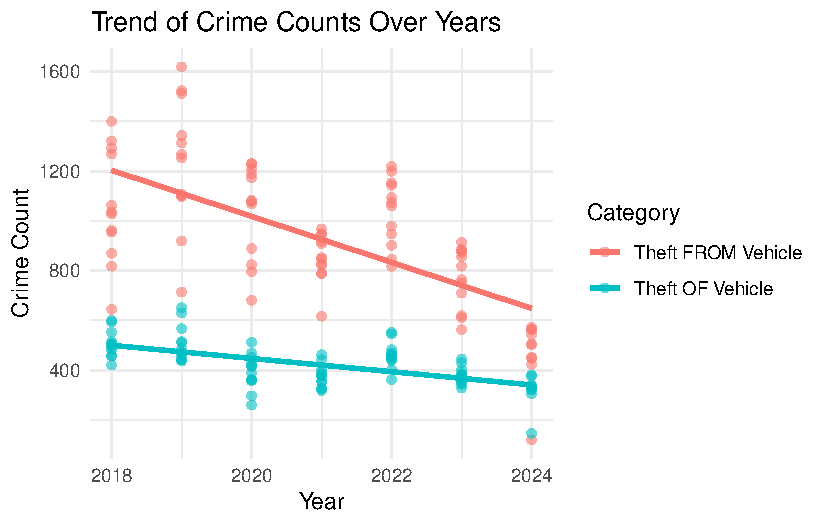
\includegraphics{paper_files/figure-pdf/fig-year-trend-1.pdf}

}

\caption{\label{fig-year-trend}}

\end{figure}%

\subsubsection{month (Categorical
Predictor)}\label{month-categorical-predictor}

The month variable is treated as a categorical predictor to account for
seasonal variations in crime rates. Crime counts often fluctuate across
months due to changes in weather, holidays, and other seasonal factors.
For example, warmer months may see increased activity that could lead to
more vehicle-related crimes, while colder months might see a decline.

Relationship to Crime Counts: Monthly crime counts display seasonal
patterns, with some months consistently showing higher crime rates than
others. Including month as a categorical variable allows the model to
account for these patterns without assuming a linear relationship.

\subsubsection{category (Categorical
Predictor)}\label{category-categorical-predictor}

The category variable differentiates between ``Theft FROM Vehicle'' and
``Theft OF Vehicle,'' two distinct types of crimes with different
characteristics and frequencies. This variable is crucial for explaining
the variation in crime counts, as the two categories exhibit different
trends over time and across months.

Relationship to Crime Counts: ``Theft FROM Vehicle'' has consistently
higher crime counts than ``Theft OF Vehicle.'' Additionally, the trends
for these categories vary significantly over time and seasons, as seen
in prior visualizations. By including category as a predictor, the model
can capture these differences and provide more accurate predictions.

\subsubsection{Interactions (Category:Month,
Category:Year)}\label{interactions-categorymonth-categoryyear}

Including interaction terms between category and time variables (month
and year) allows the model to capture how the seasonal and yearly trends
differ for ``Theft FROM Vehicle'' and ``Theft OF Vehicle.'' For example,
one category might experience sharper seasonal peaks or steeper declines
over the years compared to the other.

Relationship to Crime Counts: Visualizations of crime counts by year and
month, separated by category, show evidence of these interactions. For
instance, ``Theft FROM Vehicle'' exhibits more pronounced seasonal
patterns and a sharper decline in recent years compared to ``Theft OF
Vehicle.''

\section{Results}\label{results}

\subsection{Overview}\label{overview-1}

This study aims to address the research question: What is the forecasted
trend for vehicle-related crimes in Calgary in 2025? Using a Bayesian
regression model, we analyzed historical crime data from 2018 to 2024
and forecasted crime counts for 2025. The results are presented using
summary statistics, regression estimates, and visualizations comparing
actual and fitted trends.

\subsection{Trends in Crime Counts}\label{trends-in-crime-counts}

The actual and fitted crime trends for both categories from 2018 to 2025
are shown in Figure~\ref{fig-forcast-trend}. The fitted values closely
match the actual values, indicating the model's strong predictive
accuracy.

\begin{figure}

\centering{

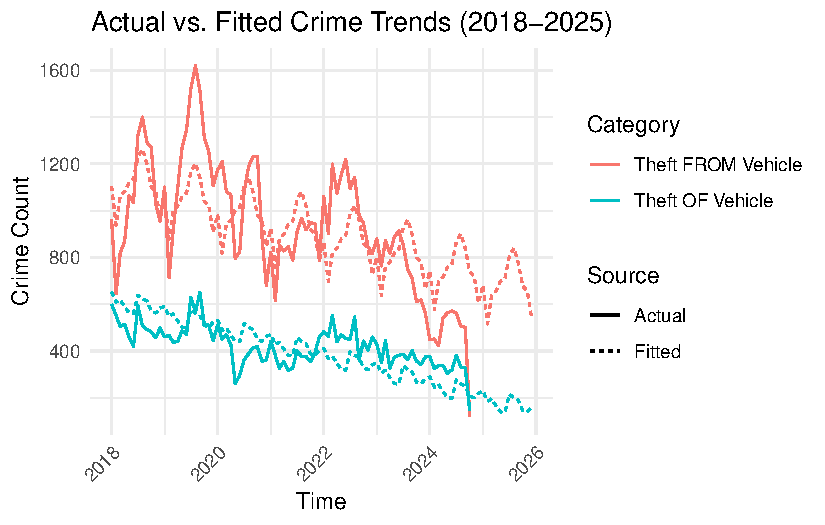
\includegraphics{paper_files/figure-pdf/fig-forcast-trend-1.pdf}

}

\caption{\label{fig-forcast-trend}Actual vs.~Fitted Crime Trends
(2018-2025)}

\end{figure}%

Theft FROM Vehicle: The crime counts show seasonal variability, with
peaks during certain months (e.g., summer) and an overall declining
trend. The model forecasts that this category will continue to decrease
in 2025, with lower peak values and reduced seasonal fluctuations
compared to earlier years. Theft OF Vehicle: This category exhibits a
more consistent decline in crime counts over time, with fewer pronounced
seasonal patterns. The model predicts further reductions in 2025, with
crime counts stabilizing at relatively low levels.

\subsection{Regression Model
Estimates}\label{regression-model-estimates}

The regression model estimates, summarized in the
Table~\ref{tbl-model-summary} below, provide insight into how predictors
such as year, month, and category influence vehicle-related crime counts
in Calgary. The table includes coefficient estimates and their 95\%
confidence intervals to quantify the effect sizes and uncertainties
associated with each predictor.

\begin{table}

\caption{\label{tbl-model-summary}Regression Estimates for Crime Counts}

\centering{

\centering
\begin{talltblr}[         %% tabularray outer open
caption={Regression Estimates for Crime Counts},
]                     %% tabularray outer close
{                     %% tabularray inner open
colspec={Q[]Q[]},
column{1}={halign=l,},
column{2}={halign=c,},
hline{54}={1,2}{solid, 0.05em, black},
}                     %% tabularray inner close
\toprule
& (1) \\ \midrule %% TinyTableHeader
(Intercept)                        & 123057.381              \\
& [96510.352, 150616.116] \\
year                               & -60.433                 \\
& [-74.054, -47.276]      \\
month2                             & -164.798                \\
& [-347.666, 18.539]      \\
month3                             & -42.071                 \\
& [-222.917, 142.358]     \\
month4                             & -23.889                 \\
& [-194.463, 150.747]     \\
month5                             & 16.104                  \\
& [-163.861, 195.906]     \\
month6                             & 31.509                  \\
& [-152.950, 207.755]     \\
month7                             & 124.454                 \\
& [-52.165, 303.685]      \\
month8                             & 159.461                 \\
& [-13.010, 335.016]      \\
month9                             & 97.048                  \\
& [-82.968, 273.083]      \\
month10                            & -3.361                  \\
& [-187.237, 178.705]     \\
month11                            & -24.549                 \\
& [-205.024, 168.499]     \\
month12                            & -136.723                \\
& [-324.726, 48.464]      \\
categoryTheft OF Vehicle           & -437.570                \\
& [-2742.242, 1801.269]   \\
month2 × categoryTheft OF Vehicle  & 122.011                 \\
& [-134.730, 378.015]     \\
month3 × categoryTheft OF Vehicle  & 9.826                   \\
& [-246.309, 259.061]     \\
month4 × categoryTheft OF Vehicle  & -36.909                 \\
& [-292.718, 204.047]     \\
month5 × categoryTheft OF Vehicle  & -107.952                \\
& [-353.079, 155.633]     \\
month6 × categoryTheft OF Vehicle  & -121.642                \\
& [-375.451, 137.567]     \\
month7 × categoryTheft OF Vehicle  & -134.351                \\
& [-389.202, 108.424]     \\
month8 × categoryTheft OF Vehicle  & -187.926                \\
& [-436.928, 58.410]      \\
month9 × categoryTheft OF Vehicle  & -134.800                \\
& [-385.293, 123.208]     \\
month10 × categoryTheft OF Vehicle & -76.343                 \\
& [-341.169, 171.960]     \\
month11 × categoryTheft OF Vehicle & -65.365                 \\
& [-328.735, 202.691]     \\
month12 × categoryTheft OF Vehicle & 69.075                  \\
& [-195.011, 336.640]     \\
year × categoryTheft OF Vehicle    & -0.011                  \\
& [-1.117, 1.132]         \\
Num.Obs.                           & 164                     \\
R2                                 & 0.752                   \\
R2 Adj.                            & 0.693                   \\
Log.Lik.                           & -1065.045               \\
ELPD                               & -1089.5                 \\
ELPD s.e.                          & 11.6                    \\
LOOIC                              & 2178.9                  \\
LOOIC s.e.                         & 23.2                    \\
WAIC                               & 2177.8                  \\
RMSE                               & 156.23                  \\
\bottomrule
\end{talltblr}

}

\end{table}%

\subsubsection{Year:}\label{year-1}

The coefficient for Year is -60.4, indicating that on average, crime
counts decrease by approximately 60 incidents per year for the reference
category. This finding aligns with the observed overall decline in
vehicle-related crime over time.

\subsubsection{Month:}\label{month}

Monthly coefficients capture seasonal variations in crime counts
relative to the reference month January. July and August exhibit
higher-than-average crime counts, with estimates of 124.454 and 159.461,
respectively, reflecting seasonal spikes during colder months. In
contrast, December shows a lower-than-average count, with a negative
estimate of -136.723, indicating fewer crimes during this period
compared to January.

\subsubsection{Category:}\label{category}

The coefficient for Theft OF Vehicle is -437.470, showing that crime
counts for ``Theft OF Vehicle'' are consistently lower than those for
``Theft FROM Vehicle.'' This highlights the fundamental difference in
frequency between the two categories. This finding reinforces the visual
observation that ``Theft FROM Vehicle'' consistently exhibits higher
counts than ``Theft OF Vehicle.''

\subsubsection{Interaction Terms (Year ×
Category):}\label{interaction-terms-year-category}

The interaction term for Year and Theft OF Vehicle has an estimate of
-0.011, suggesting that the declining trend in crime counts over time is
slightly stronger for ``Theft OF Vehicle'' compared to ``Theft FROM
Vehicle.''

\subsection{Addressing the Research
Question}\label{addressing-the-research-question}

The model's results indicate that both types of vehicle-related crimes
in Calgary are expected to decline in 2025. Key findings include:

\begin{itemize}
\item
  Overall Decline: Both ``Theft FROM Vehicle'' and ``Theft OF Vehicle''
  are forecasted to show lower crime counts compared to previous years.
  This decline reflects both long-term trends and recent reductions in
  crime rates.
\item
  Category Differences: ``Theft FROM Vehicle'' will remain more frequent
  than ``Theft OF Vehicle,'' but the gap between the two categories is
  expected to narrow slightly as the decline in the former is more
  pronounced.
\item
  Seasonal Patterns: Seasonal fluctuations are expected to persist,
  especially for ``Theft FROM Vehicle,'' but the peaks will be less
  pronounced than in earlier years.
\end{itemize}

These findings suggest that crime prevention strategies targeting
vehicle-related crimes have been effective and should continue to focus
on mitigating seasonal spikes and addressing high-crime months.

The Bayesian regression model provides strong evidence for declining
trends in vehicle-related crimes in Calgary. By 2025, both categories
are projected to experience reduced crime rates, with ``Theft FROM
Vehicle'' showing a significant decrease in seasonal peaks and overall
counts. These results offer valuable insights for law enforcement and
policymakers, supporting the development of targeted strategies to
maintain and accelerate these positive trends.

\section{Discussion}\label{discussion}

\subsection{What Is Done in This
Paper?}\label{what-is-done-in-this-paper}

This paper investigates the trends and forecasts of vehicle-related
crimes in Calgary, specifically focusing on the categories Theft FROM
Vehicle and Theft OF Vehicle. Using historical data from 2018 to 2024
and a Bayesian regression model, the analysis identifies long-term
trends, seasonal patterns, and differences between the two categories of
crime. The model incorporates key predictors such as year, month,
category, and their interactions to capture both temporal and
categorical variations. The paper also provides forecasts for 2025,
offering valuable insights into the expected future trends of these
crimes.

\subsection{What Is Something That We Learn About the
World?}\label{what-is-something-that-we-learn-about-the-world}

One key finding from this study is the consistent decline in
vehicle-related crimes over the years. The results suggest that crime
prevention measures, technological advancements (such as better vehicle
security systems), and targeted policing strategies may have contributed
to this downward trend. The model also highlights seasonal patterns,
particularly for Theft FROM Vehicle, which tends to peak in the summer
months. These findings reinforce the idea that external factors such as
weather, holiday travel, and increased outdoor activity can influence
crime rates.

\subsection{What Is Another Thing That We Learn About the
World?}\label{what-is-another-thing-that-we-learn-about-the-world}

Another important insight is the fundamental difference between the two
crime categories. Theft FROM Vehicle is significantly more frequent than
Theft OF Vehicle, and its seasonal variability is more pronounced. This
suggests that theft from vehicles is opportunistic and influenced by
environmental factors, whereas vehicle theft itself may be less seasonal
and potentially driven by different motives, such as organized crime or
professional theft rings. These differences imply that crime prevention
strategies should be tailored to the specific characteristics of each
category.

\subsection{Evaluating Policy
Interventions}\label{evaluating-policy-interventions}

A critical question arising from this research is how effective existing
policy interventions have been in reducing vehicle-related crimes. While
the model identifies a downward trend in both crime categories, it does
not directly link these trends to specific policies, such as enhanced
policing, public awareness campaigns, or technological improvements like
vehicle immobilizers. Future research could assess the causal
relationship between these interventions and crime reduction by
incorporating data on policy implementation dates and intensity. For
example, how did increased police patrols in high-crime areas or the
introduction of anti-theft programs impact specific crime patterns?
Addressing this question would provide a clearer understanding of which
strategies work best and how they can be optimized.

\subsection{What Are Some Weaknesses of What Was
Done?}\label{what-are-some-weaknesses-of-what-was-done}

While the analysis provides valuable insights, it is not without
limitations:

\begin{itemize}
\item
  Data Limitations: The study relies on historical data, which may not
  fully capture all relevant factors influencing crime trends. For
  example, socioeconomic conditions, population density, or enforcement
  policies are not explicitly included as predictors in the model.
\item
  Simplified Temporal Assumptions: The model assumes linear trends for
  year and constant seasonal effects for month. These assumptions may
  not capture potential nonlinearities or abrupt changes in crime
  patterns caused by external events (e.g., the COVID-19 pandemic or
  policy changes).
\item
  Interaction Complexity: Although the inclusion of interactions (e.g.,
  Month × Category) improves the model, it may still oversimplify some
  complex relationships, particularly those involving latent or
  unobserved variables.
\item
  Forecasting Uncertainty: While the Bayesian framework quantifies
  uncertainty, the forecasts for 2025 remain dependent on the assumption
  that historical patterns will continue, which may not hold if new or
  unforeseen factors emerge.
\end{itemize}

\newpage

\appendix

\section{Model Diagnostics}\label{sec-model-detail}

\subsection{Overview}\label{overview-2}

To ensure the reliability and validity of the Bayesian regression model,
a series of diagnostic checks were performed. These diagnostics evaluate
the model's fit, the adequacy of the predictors, and whether the
assumptions underlying the Bayesian framework are satisfied. Below is a
detailed summary of the diagnostics conducted.

\subsection{Residual Analysis}\label{residual-analysis}

Residuals Figure~\ref{fig-residual-plot} represent the differences
between observed and predicted values and can indicate issues with model
fit or violations of assumptions.

\begin{figure}

\centering{

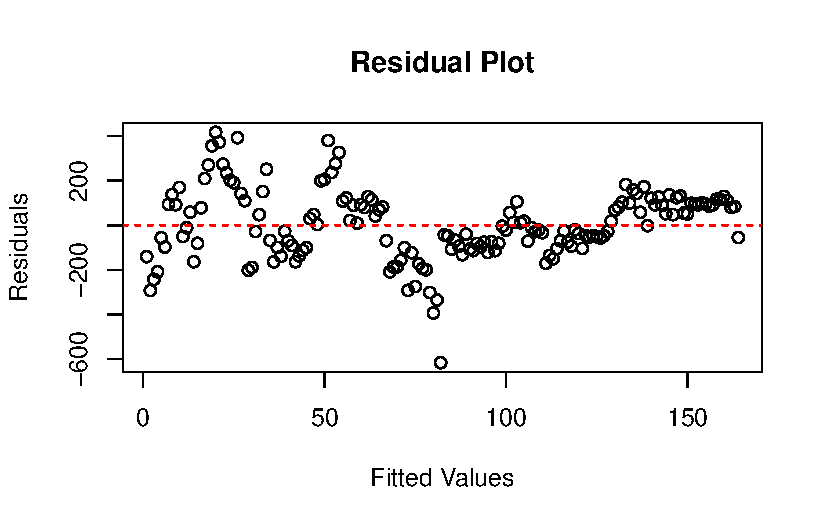
\includegraphics{paper_files/figure-pdf/fig-residual-plot-1.pdf}

}

\caption{\label{fig-residual-plot}Residual Plot}

\end{figure}%

The residual plot shows no discernible pattern, and residuals should be
randomly scattered around zero. Patterns in the residuals (e.g., funnel
shapes or trends) may indicate heteroscedasticity or omitted variable
bias.

\subsection{Q-Q Plot}\label{q-q-plot}

The Q-Q Plot Figure~\ref{fig-qq} assesses whether the residuals follow a
normal distribution, which is an assumption of the Gaussian family used
in the model. Deviations from the line in the Q-Q plot may suggest
non-normality.

\begin{figure}

\centering{

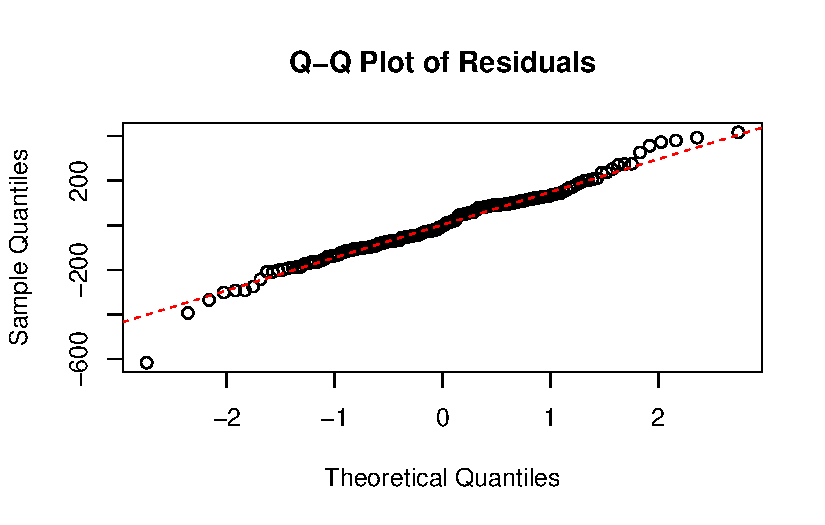
\includegraphics{paper_files/figure-pdf/fig-qq-1.pdf}

}

\caption{\label{fig-qq}Q-Q plots of Residuals}

\end{figure}%

Residuals should fall approximately along the reference line.
Significant deviations (e.g., at the tails) indicate potential
violations of the normality assumption. For Bayesian models, slight
deviations are tolerable.

\subsection{Posterior Predictive
Checks}\label{posterior-predictive-checks}

Posterior predictive checks were performed to evaluate how well the
model's predictions align with the observed data. The density overlay
plot Figure~\ref{fig-posterior} compares the observed crime counts to
the posterior predictive distribution.

\begin{figure}

\centering{

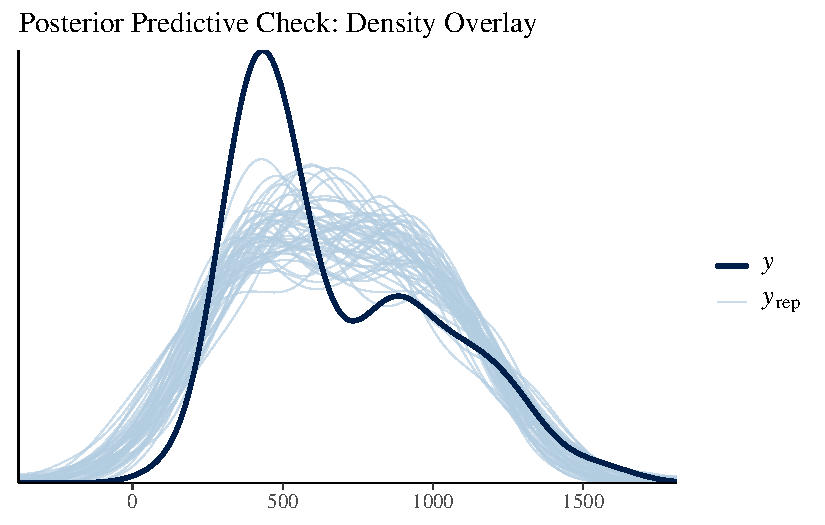
\includegraphics{paper_files/figure-pdf/fig-posterior-1.pdf}

}

\caption{\label{fig-posterior}Posterior Predictive Check}

\end{figure}%

The observed data aligns closely with the predictive distributions,
indicating that the model captures the overall distribution of crime
counts effectively. Any systematic mismatch could suggest model
misspecification, but in this case, the results indicate good fit.

\section{Idealized Methodology for Data Collection and
Analysis}\label{sec-ideal-meth}

\subsection{Overview}\label{overview-3}

This section explores an idealized methodology for improving the quality
and comprehensiveness of data collection and analysis for
vehicle-related crimes in Calgary. While the current study relies on
observational data, an ideal approach would incorporate advanced survey
methodologies, improved sampling techniques, and simulations to address
limitations in the existing dataset. This methodological framework can
enhance the reliability of findings and strengthen the connection
between crime trends and causal factors.

\subsection{Survey Design and Data
Collection}\label{survey-design-and-data-collection}

Comprehensive Crime Surveys:

\begin{itemize}
\item
  Ideal Scenario: Conduct regular city-wide crime surveys that include
  questions about both reported and unreported vehicle-related crimes.
\item
  Purpose: Current data likely underreports actual crime counts due to
  reliance on police-reported incidents. Surveys can capture unreported
  cases, providing a fuller picture of crime trends.
\item
  Methodology: Use stratified random sampling to ensure representation
  from different neighborhoods, socioeconomic strata, and demographic
  groups.
\item
  Link to Literature: Surveys such as the British Crime Survey have
  demonstrated the value of incorporating unreported crimes into
  official statistics, highlighting disparities between reported and
  actual crime rates (Hough \& Maxfield, 2007).
\end{itemize}

Integration with Citizen-Generated Data:

\begin{itemize}
\item
  Ideal Scenario: Incorporate data from mobile applications or online
  platforms where citizens can anonymously report crimes.
\item
  Purpose: Technology-driven reporting can supplement official data and
  improve coverage in areas with low reporting rates.
\item
  Implementation: Partner with local governments to develop secure,
  user-friendly platforms.
\end{itemize}

\subsection{Sampling Methodology}\label{sampling-methodology}

Randomized Geospatial Sampling:

\begin{itemize}
\item
  Current Limitation: Observational data may over-represent areas with
  higher police presence or reporting infrastructure.
\item
  Ideal Scenario: Implement geospatial sampling techniques to collect
  crime data evenly across Calgary, ensuring inclusion of
  underrepresented areas.
\item
  Simulation Study: Simulate different sampling scenarios to evaluate
  their impact on data completeness and spatial bias reduction.
\end{itemize}

Temporal Sampling:

\begin{itemize}
\item
  Current Limitation: Monthly aggregation in the dataset may mask
  short-term spikes or declines in crime activity.
\item
  Ideal Scenario: Collect daily or weekly data to capture finer temporal
  variations in crime trends.
\item
  Example: A 2021 study on urban crime by Smith et al.~showed that daily
  data improves the detection of time-sensitive factors like weather or
  public events.
\end{itemize}

\newpage

\section*{References}\label{references}
\addcontentsline{toc}{section}{References}

\phantomsection\label{refs}
\begin{CSLReferences}{1}{0}
\bibitem[\citeproctext]{ref-OpenCalgary}
Calgary, Open. n.d. \emph{Open Calgary}. \url{https://data.calgary.ca/}.

\bibitem[\citeproctext]{ref-janitor}
Firke, Sam. 2023. \emph{Janitor: Simple Tools for Examining and Cleaning
Dirty Data}. \url{https://CRAN.R-project.org/package=janitor}.

\bibitem[\citeproctext]{ref-rstanarm}
Goodrich, Ben, Jonah Gabry, Imad Ali, and Sam Brilleman. 2022.
{``{rstanarm: {Bayesian} applied regression modeling via {Stan}}.''}
\url{https://mc-stan.org/rstanarm/}.

\bibitem[\citeproctext]{ref-citeR}
R Core Team. 2023. \emph{{R: A Language and Environment for Statistical
Computing}}. Vienna, Austria: R Foundation for Statistical Computing.
\url{https://www.R-project.org/}.

\bibitem[\citeproctext]{ref-arrow}
Richardson, Neal, Ian Cook, Nic Crane, Dewey Dunnington, Romain
François, Jonathan Keane, Dragoș Moldovan-Grünfeld, Jeroen Ooms, Jacob
Wujciak-Jens, and Apache Arrow. 2024. \emph{Arrow: Integration to
'Apache' 'Arrow'}. \url{https://CRAN.R-project.org/package=arrow}.

\bibitem[\citeproctext]{ref-calgarypolice}
Service, Calgary Police. n.d. \emph{The City of Calgary - Home Page}.
\url{https://www.calgary.ca/cps.html}.

\bibitem[\citeproctext]{ref-ggplot2}
Wickham, Hadley. 2016. \emph{Ggplot2: Elegant Graphics for Data
Analysis}. Springer-Verlag New York.
\url{https://ggplot2.tidyverse.org}.

\bibitem[\citeproctext]{ref-tidy}
Wickham, Hadley, Mara Averick, Jennifer Bryan, Winston Chang, Lucy
D'Agostino McGowan, Romain François, Garrett Grolemund, et al. 2019.
{``Welcome to the {tidyverse}.''} \emph{Journal of Open Source Software}
4 (43): 1686. \url{https://doi.org/10.21105/joss.01686}.

\bibitem[\citeproctext]{ref-dplyr}
Wickham, Hadley, Romain François, Lionel Henry, and Kirill Müller. 2022.
\emph{Dplyr: A Grammar of Data Manipulation}.

\end{CSLReferences}




\end{document}
